\Lecturer{Hui Jin}
\Contributor{}
\LectureNumber{07}
\LectureDate{DATE}
\LectureTitle{Turbo Codes}

\lstset{style=mystyle}

	\MakeScribeTop

%#############################################################
%#############################################################
%#############################################################
%#############################################################

\section{Introduction}
In late 1980s, there was a sense that "channel coding" was a dead field. Algebraic codes like Reed Solomon codes and convolutional codes had been studied thoroughly. They showed good performance but fell well short of the Shannon limit.  In fact, the best codes usually required more than twice the transmitting power that Shannon’s law said was necessary to reach a certain level of reliability. The gap between the practical and the ideal, measured in decibels — a ratio between the signal level and the noise level on a logarithmic scale — was about $3.5$ dB. To chip away at it, engineers needed more elaborate codes. On other channels, like block fading channels, the gap was even wider. But there seemed a dead end for new ideas. A lot of researchers believed that the $3$dB barrier to the Shannon limit was unbreakable.


Then, completely out of the blue, a revolution in coding theory occurred in 1993. On the IEEE International Communications Conference, French researchers Berrou and Glavieux presented a new type of codes - turbo codes. The researchers claimed that these codes could achieve within $1$dB of the Shannon capacity. On this outlandish claim, many in the conference were skeptical, partially because at the time the authors of the paper were largely unknown in the field. Few people bothered to read the paper, suspecting the authors made some calculation error in the units of signal-to-noise ratio. But once other researchers began to validate the results independently, a massive research effort was soon underway with the goal of explaining and, better yet, enhancing the remarkable performance of turbo codes. Much of this research focused on improving the practicality of turbo codes, which, as will be dis- cussed shortly, have some peculiarities that make implementation less than straightforward.

By the end of the 1990s, the virtues of turbo codes were well known, and they began to be adopted in various systems. Now they are incorporated into standards used by NASA for deep space communications (CCSDS), and both third-generation cellular standards (UMTS and cdma2000).


\section{Turbo Code Structure}
The original turbo code was the parallel concatenated convolutional code (PCCC). 

\subsection{Recursive Systematic Convolutional Code}
In inventing Turbo codes, Dr. Berrou was also the first one to introduce Recursive Systematic Convolutional Codes. 

The RSC encoder of this conventional convolutional encoder is represented 12
as \(G=[1, g / g ]\) where the first output (represented by g ) is fed back to the input.  Figure \ref{fig:Conv_RSC} shows the resulting 
RSC encoder.

\begin{figure}[h]
    \centering
    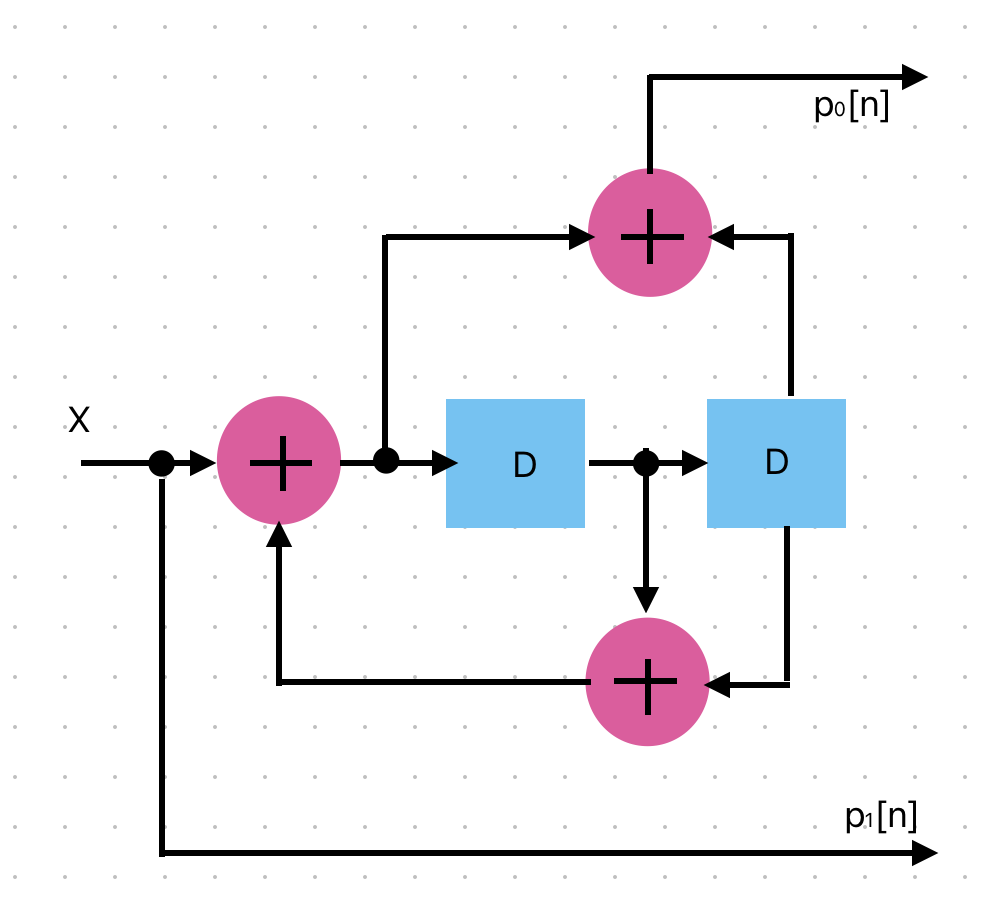
\includegraphics[width=0.6\textwidth]{Figs/Conv_RSC.png}
    \caption{Caption}
    \label{fig:Conv_RSC}
\end{figure}

\subsection{Transfer Function of RSC}
The transfer function of the code defined in Fig~\ref{fig:Conv_RSC}.
We will introduce the variable \(s[n]\) to represent the value right before first register. Then we have the following equations: 
\begin{align*}
s[n] = x[n] + s[n-1] + s[n-2] \nonumber
p[n] = s[n] + s[n-2]
\end{align*}
Applying the \(z\)-transform to the two equations, we have 
\begin{align*}
S(1+z + z^2) &= X, \\
P &= S(1 + z^2).
\end{align*}
Canceling \(S\) in the above two equations gives us the transfer function: 

\begin{align}
\frac{P}{X} = \frac{1+z^2}{1+ z + z^2} \label{eq:RSCTransfer}
\end{align}

Compared with a non-recursive convolutional code, the transfer function of a recursive convolutional code has a non constant denomintor function. This provides the feedback loop.

\subsection{Turbo Code Structure}

\subsection{Encoding}

\subsection{Puncturing}

structure and the encoding algorithm. 
\section{Interleaver Design}
\subsection{Random Interleaver} 
\subsection{S-random interleaver}

\section{Serial Turbo Code}


\section{Irregular Turbo Code}

Algebraic construction. 


